\documentclass[letterpaper,11pt]{article}
\usepackage{graphicx}
\usepackage{listings}
\usepackage[super]{nth}
\usepackage[hyphens]{url}
\usepackage{hyperref}
\usepackage{amsmath}
\usepackage[makeroom]{cancel}
\usepackage[table]{xcolor}
\usepackage{comment}
\usepackage[space]{grffile}
\usepackage{csvsimple}
\usepackage{longtable}
\usepackage{adjustbox}


\newcommand*{\srcPath}{../src}%

\lstset{
	basicstyle=\footnotesize,
	breaklines=true,
}

\begin{document}

\begin{titlepage}

\begin{center}

\Huge{Assignment 2}

\Large{CS 734:  Introduction to Information Retrieval}

\Large{Fall 2017}

\Large{Grant Atkins}

\Large Finished on \today

\end{center}

\end{titlepage}

\newpage


% =================================
% First question
% =================================
\section*{1}

\subsection*{Question}

\begin{verbatim}
1.2 	Site Search is another common application of search engines.
In this case, search is restricted to the web pages at a given website.
Compare site search to web search, vertical search, and enterprise search.
\end{verbatim}

\subsection*{Answer}

To answer this question I decided to use the search query ``cs834-f17'' with modifications as necessary across each of these search types.
For site search I used github.com as our course repository is hosted on github and will likely return results and as the name site search implies it only searches on the designated website.
Google offers the option to site search with the command ``site:website'' which for my entry it is ``cs834-f17 site:github.com''  as shown in Figure \ref{fig:sitesearch} \cite{googlesite}.
It only returned two results which is minimal and as expected because it is a unique term and the term ``cs834-f17'' isn't expected to be located in any other repository or description hosted on github.

For web search I continued to use google. Using the query term ``cs834-f17'' this time without specifying anything else returned 57 results as shown in Figure \ref{fig:websearch}.
Both web search and site search both return the same top result, which is the repository. Something that is interesting in this search is that it didn't show the second result
from the site search. Instead the web search went to different domains to try and find ``cs834-f17'', for example \textit{github.io}. This should be noted as the precision in site search
is seems to be more effective in the context of terms.

Continuing with vertical search I also made use of google images. The goal of vertical search is to search on a specific content type.
The results were somewhat expected as there was in fact a picture of the author of the cs834-f17 repository, Dr. Nelson as shown in Figure \ref{fig:verticalsearch}, however prior to that image it seems of had lot of patent schemes for protein formulas. In this context it probably wasn't the best to use a vertical search.

Finally when completing Enterprise search it should be noted that I don't have access to an intranet but I do have access to my own personal machine to conduct searches on my own file system.
I used my operating system's implemented search in it file system and I also use the terminal command \textit{grep} to show a customized search on a subset of directories.
Using my operating systems \textit{finder} program it searches across my entire computer of files with the words ``cs834-f17'' as shown in Figure \ref{fig:esearch1}. This type of seems more relatable to web search as it seem to generalize the results showing files that mention this term, but not every single file in my filesystem.
When I used the \textit{grep} command searching any directories starting with ``cs'' it showed every occurrence where ``cs834-f17'' was used. This is more relatable to site search because it listed all locations of occurrence in these directories.

  \begin{figure}[h]
  \centering
  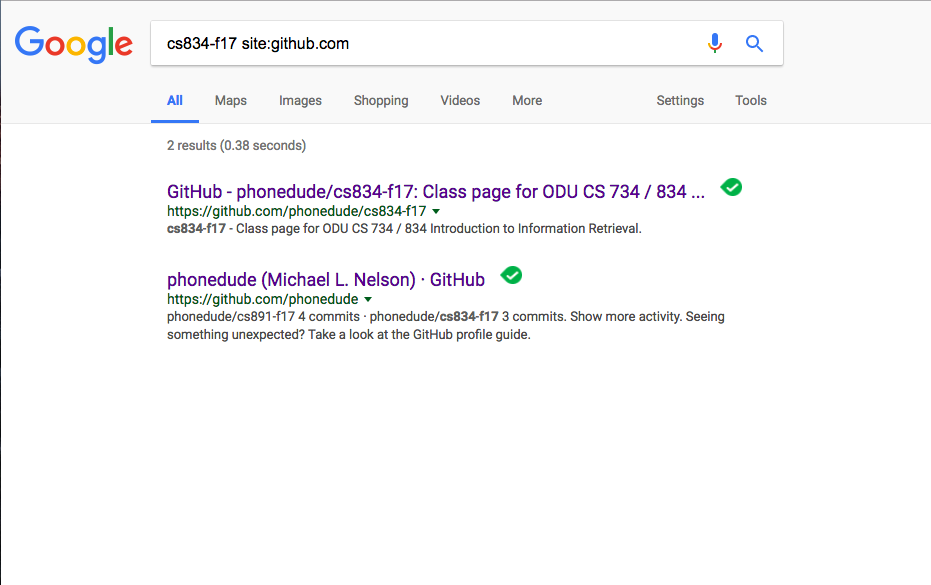
\includegraphics[scale=0.4]{sitesearch.png}
  \caption{Site search example in google}
  \label{fig:sitesearch}
  \end{figure}


\clearpage

% =================================
% Second question
% =================================

\section*{2}

\subsection*{Question}

\begin{verbatim}
1.4 	List five web services or sites that you use that appear to use search,
not including web search engines. Describe the role of search for that
service. Also describe the search is based on a database or grep style
of matching, or if the search is using some type of ranking.
\end{verbatim}

\subsection*{Answer}


\clearpage

% =================================
% 3rd question
% =================================

\section*{3}

\subsection*{Question}

\begin{verbatim}
3.7 	Write a program that can create a valid sitemap based on the
contents of a directory on your computer's hard disk. Assume
the file are accessible from a website at the URL http://example.com.
For instance, if there is a file in your directory called homework.pdf,
this would be available at http://www.example.com/homework.pdf.
Use the real modification date on the file as the last modified time in the
sitemap, and to help estimate the change frequency.
\end{verbatim}

\subsection*{Answer}


 \lstinputlisting[frame=single,caption={Python script create a sitemap from a directory's contents},label=lst:sitemap,captionpos=b,numbers=left,showspaces=false,showstringspaces=false,basicstyle=\footnotesize]{\srcPath/sitemap.py}

\clearpage

% =================================
% 4th question
% =================================

\section*{4}

\subsection*{Question}

\begin{verbatim}
Suppose that, in an effort to crawl web pages faster, you set up
two crawling machines with different starting seed URIs. Is this
an effective strategy for distributed crawling? Why or why not.
\end{verbatim}

\subsection*{Answer}


\clearpage

% =================================
% 5th question
% =================================

\section*{5}

\subsection*{Question}

\begin{verbatim}
3.9 	Write a simple single-threaded web crawler. Starting from a single input
URL (perhaps a professor's web page), the crawler should download a
page and then wait at least five seconds before downloading the next
page. Your program should find other pages to crawl by parsing link
tags found in previously crawled documents.
\end{verbatim}

\subsection*{Answer}


\clearpage


% =================================
% Bibliography
% =================================

\begin{thebibliography}{9}
\bibitem{cs532}
Atkins, Grant. ``CS532 Assignment 1 Repository'' Github. N.p., 23 March 2017. Web. 23 March 2017.\url{https://github.com/grantat/cs532-s17/tree/master/assignments/A1/src}.
\bibitem{github}
Atkins, Grant. ``CS734 Assignment 2 Repository'' Github. N.p., 21 September 2017. Web. 21 September 2017.\url{https://github.com/grantat/cs834-f17/tree/master/assignments/A2}.
\end{thebibliography}

\end{document}
